\chapter{Ergebnisse}
\label{chap:results}
In diesem Kapitel werden die Ergebnisse der durchgeführten Experimente präsentiert. Zuerst wird die Eignung der Themenmodelle präsentiert. Anhand der Resultate werden die Themenmodelle ausgewählt, die dazu genutzt werden, die Themenverläufe zu erstellen. Anschließend werden die Ergebnisse der Evaluation der Zentralitätsindizes vorgestellt und die Themenverläufe der realen Textsequenzen abgebildet und diskutiert.  

\section{Evaluation der Themenmodelle}
\label{sec:tmValResults}

\subsection{SCY-Chatdaten}
Für die SCY-Daten wurden zuerst Themenmodelle gelernt, die jeweils 5 bis 100 Themen enthalten. Ab einer Themenanzahl von 15 wurde nur jedes fünfte Modell gelernt, so wurden Modelle mit von 2-15 Themen, 20 Themen, 25 Themen, usw. gelernt. Dabei wurden verschiedene Parameter variiert. Zum einen wurden Stopwörter aus dem Trainingskorpus entfernt, zum anderen wurden die Terme auf ihre Stammform reduziert. Die Parameter $\alpha$ und $\beta$ wurden auf Werte gesetzt, die im Allgemeinen gute Modelle ergeben \citep{Griffiths2004LDA}. Dies ist $\alpha=50/K$ mit $K = \text{Anzahl der Themen}$ und $\beta=0.01$. So wurden insgesamt vier Sätze von Themenmodellen gelernt.  

\begin{figure}
  \subfigure[Themenmodelle ohne Stammformreduktion] {
    \label{fig:tmEvalNoStemStop}
    \includegraphics[width=0.98\textwidth,height=0.4\textheight]{images/content/06_results/co2_nostem} 
  }
  \subfigure[Themenmodelle mit Stammformreduktion]{
    \label{fig:tmEvalStemStop}
    \includegraphics[width=0.98\textwidth,height=0.4\textheight]{images/content/06_results/co2_stem} 
  }
\caption{Evaluationsergebnisse der Themenverläufe mit Stopwortentfernung für das SCY-Korpus. Es sind Mittelwert und Varianz aller Evaluationsdurchgänge abgetragen}
\label{fig:topicModelEvaluationStop}
\end{figure}

Ein Satz von Modellen, in denen nur die Stopwörter entfernt wurden, ein Satz von Modellen, in denen sowohl Stopwörter entfernt wurden als auch die Terme auf ihre Grundform reduziert wurden, ein Satz von Modellen, bei denen die Terme nur auf ihre Grundform reduziert wurden und ein Satz von Modellen, bei denen weder die Stopwörter entfernt wurden als auch keine Grundformreduktion vorgenommen wurde. Auf jedes Modell in einem Satz wurde die in Abschnitt \ref{sec:topicValidation} erläuterte Validationsmethode angewendet. Für jedes Modell in einem Satz erhält man so eine Bewertungszahl. 

Da sich die Ergebnisse des Approximationsalgorithmus, der verwendet wurde um die Themenmodelle zu lernen, in Abhängigkeit von den für den Gibbs-Sampler gewählten Startwerten geringfügig unterscheiden, wurden die verschiedenen Sätze insgesamt fünfmal neu gelernt. Dann wurde der Mittelwert und die Varianz aller fünf Evaluationsdurchgänge bestimmt. So sollen eventuelle Schwankungen bei der Approximation der Themen- und Termverteilungen ausgeglichen werden. Die berechneten Mittelwerte und Varianz wurden gegen die Anzahl der Themen in ein Diagramm eingetragen. Daraus kann man ablesen, welche Themenmodelle die geeignetsten sind, um möglichst klar voneinander abgegrenzte Themen zu erhalten. Für die verschiedene Sätze von Themenmodellen sind die Ergebnisse der Evaluation in Abbildung \ref{fig:topicModelEvaluationStop} und Abbildung \ref{fig:topicModelEvaluationNoStop} dargestellt. 

\begin{figure}
\subfigure[Themenmodelle ohne Stammformreduktion]{
    \label{fig:tmEvalNoStemNoStop}
    \includegraphics[width=0.98\textwidth,height=0.4\textheight]{images/content/06_results/co2_nostem_nostop} 
  }
  \subfigure[Themenmodelle mit Stammformreduktion]{
    \label{fig:tmEvalStemNoStop}
    \includegraphics[width=0.98\textwidth,height=0.4\textheight]{images/content/06_results/co2_stem_nostop} 
  }  
\caption{Evaluationsergebnisse der Themenverläufe ohne Stopwortentfernung für das SCY-Korpus. Es sind Mittelwert und Varianz aller Evaluationsdurchgänge abgetragen}
\label{fig:topicModelEvaluationNoStop}
\end{figure}

Für alle Konfigurationen der Modelle steigt die Kullback-Leibler-Divergenzen stark an, hält sich kurzzeitig auf einem Plateau und fällt dann wieder ab. Das Plateau zeigt die optimale Anzahl der Themen an. Für die Modelle, die ohne Stammformreduktion trainiert wurden, ist erkennbar, dass die beste Themenanzahl im Bereich von 10 bis 25 Themen liegt. Für den Satz von Modellen, die mit Stammformreduktion der Terme gelernt wurden, wird eine höhere Kullback-Leibler-Divergenz erreicht. Für diese Modelle wird die optimale Themenanzahl um ca. fünf Themen nach oben verschoben. Die optimale Themenanzahl bewegt sich somit zwischen 15 und 30.

Alle Themenmodelle, deren Themenanzahl kleiner als zehn ist, repräsentieren die Hintergrundtexte nicht gut, da zu wenig Themen ausgewählt wurden, um die Komplexität der Texte zu erfassen. Die extrahierten Themen sind zu vage, um klar von einander abgegrenzt zu werden. Entsprechend ist es für Themenmodelle mit Anzahl der Themen größer als 25. Für diese werden die Terme auf zu viele Themen aufgeteilt. Die Themen werden zu speziell und somit auch nicht mehr interpretierbar. 

\subsection{dpa Nachrichtenmeldungen}
\begin{figure}
  \subfigure[Themenmodelle ohne Stammformreduktion]{
    \label{fig:dpaTmEvalNoStemStop}
    \includegraphics[width=0.98\textwidth,height=0.4\textheight]{images/content/06_results/dpa_nostem} 
  }
  \subfigure[Themenmodelle mit Stammformreduktion]{
    \label{fig:dpaTmEvalStemStop}
    \includegraphics[width=0.98\textwidth,height=0.4\textheight]{images/content/06_results/dpa_stem} 
  }
\caption{Evaluationsergebnisse der Themenverläufe mit Stopwortentfernung für das dpa-Korpus. Es sind Mittelwert und Varianz aller Evaluationsdurchgänge abgetragen}
\label{fig:dpaTopicModelEvaluationStop}
\end{figure}

Für das dpa-Korpus wurden analog Themenmodelle mit einer Anzahl von 10 bis 200 Themen gelernt, wobei nur für jede zehnte Themenanzahl ein Modell gelernt wurde. Eine Ausnahme liegt im Bereich von 30 bis 40 Themen. Hier wurde jedes Themenmodelle gelernt, um das genaue Verhalten der Evaluationsmaße in diesem lokalen Bereich zu bestimmen. Es wurden auch wieder mehrere Sätze von Modellen gelernt, die sich durch die Parameter unterscheiden. Wie für das SCY-Korpus wurden Stopwörter entfernt und die Terme auf ihre Stammform reduziert. Die Parameter $\alpha$ und $\beta$ wurden auf den Standardwerten belassen. Jeder Satz wurde insgesamt fünfmal anhand desselben Korpus und derselben Parameter neu gelernt. Aus den ermittelten Kullback-Leibler Divergenzwerten für die einzelnen Modelle wurde der Mittelwert und die Varianz berechnet. Diese wurden dann auch gegen die Themenanzahl aufgetragen. Die resultierenden Diagramme sind in Abbildung \ref{fig:dpaTopicModelEvaluationStop} und Abbildung \ref{fig:dpaTopicModelEvaluationNoStop} zu sehen.

Die Kurven zeigen das schon bei den SCY-Modellen gesehene Verhalten. Sie steigen recht schnell an, bewegen sich dann kurzzeitig auf einem Plateau und fallen dann wieder ab. Auch hier zeigt das Plateau die optimalen Anzahl von Themen an. Der optimale Bereich liegt für die Modelle, die ohne Stammformreduktion gelernt wurden, zwischen 40 und 70 Themen. Für die Modelle, die eine Stammformreduktion der Terme beinhalten, liegt der optimale Bereich zwischen 50 und 90. 

Interessant ist der Bereich zwischen 30 und 40. Die Kurve weist hier starke Schwankungen bei hoher Varianz auf. Zum einen lassen sich die Schwankungen damit erklären, dass die Sätze nur fünfmal neu gelernt werden. Würden die Sätze öfter neu gelernt, würde der Mittelwert sich wahrscheinlich dem idealen Verlauf der Kurve annähern. Andererseits schwanken die Kullback-Leibler-Werte aufgrund des verwendeten Approximationsalgorithmus für die Themen- und Termverteilungen. Der Gibbs-Sampling Algorithmus weist die Terme den Themen zufällig zu. Zwar konvergiert der Algorithmus gegen die gesuchte Verteilung, es kann dabei aber zu Schwankungen bei der Zuweisung von Termen zu Themen, kommen. So ist es möglich, dass die Themenanzahl einmal eine gute Trennung der Themen ergibt und in einem andern Fall keine gute Trennung erreicht wird. Dieser Effekt tritt bei den SCY-Texten nicht auf. Dies kann an der Anzahl von Termen im Korpus liegen. Da im SCY-Korpus nur ca. 8.000 Terme unterschieden werden und im dpa-Korpus mehr als 100.000 Terme vorhanden sind, können größere Schwankungen auftreten. Dies genauer zu untersuchen, würde jedoch den Fokus der Diplomarbeit verlassen. 

\begin{figure}
\subfigure[Themenmodelle ohne Stammformreduktion]{
    \label{fig:dpaTmEvalNoStemNoStop}
    \includegraphics[width=0.98\textwidth,height=0.4\textheight]{images/content/06_results/dpa_nostem_nostop} 
  }
  \subfigure[Themenmodelle mit Stammformreduktion]{
    \label{fig:dpaTmEvalStemNoStop}
    \includegraphics[width=0.98\textwidth,height=0.4\textheight]{images/content/06_results/dpa_stem_nostop} 
  }  
\caption{Evaluationsergebnisse der Themenverläufe ohne Stopwortentfernung für das dpa-Korpus. Es sind Mittelwert und Varianz aller Evaluationsdurchläufe abgetragen}
\label{fig:dpaTopicModelEvaluationNoStop}
\end{figure}

Generell kann man sagen, dass die optimale Anzahl der Themen steigt, wenn eine Stammformreduktion durchgeführt wird. Die Entfernung der Stopwörter hat hingegen keinen Einfluss auf die Eignung der Themenmodelle. 

\section{Evaluation der Zentralitätsverläufe}
\label{sec:centralityResults}

Anhand der in Abschnitt \ref{sec:tmValResults} als geeignet identifizierten Themenmodelle und der synthetisch erstellten Dokumentverläufe werden nun die Zentralitätsmaße zusammen mit dem Graphenalgorithmus ermittelt, die geeignet sind die Themenveränderung wiederzugeben. Dazu wurden, wie schon in Abschnitt \ref{sec:centralityEvaluation} beschrieben, die Themenverläufe für die synthetisch erstellten Dokumente ermittelt und anhand des F-Maßes bewertet wie gut diese erfasst und repräsentiert werden. Der Schwellwert $t$ wurde dabei auf $1.0$ gesetzt. Von den für jedes Modell berechneten F-Werten wird dann wiederum der Mittelwert bestimmt. 

Für jeden in Abschnitt \ref{sec:topic2graph} erläuterten Algorithmus wird so eine Tabelle erstellt, die anzeigt welches Zentralitätsmaß, welchen Verlauf wie gut erfasst. Die Tabellen werden noch nach den Parametern des zugrundeliegenden Themenmodells unterschieden. Es werden also pro Korpus zwölf Tabellen erstellt. Wenn sich die Werte der mit verschiedenen Parametern trainierten Modelle nicht signifikant unterscheiden, wird aus Platzgründen nur eine Tabelle pro Algorithmus dargestellt. 

\subsection{SCY-Chatdaten}

Für die synthetischen SCY-Chatdaten unterscheiden sich die Bewertungen der einzelnen Sätze nicht signifikant. Es werden deshalb nur die Ergebnisse jeweils eines Modellsatzes präsentiert. 
\begin{table}[!ht]
\centering
\begin{tabular}[ht]{l|c|c|c|c|c|c|c|c|c}
\hline
\hline
	& $\centrality{B}$	& $\centrality{C}$	& $\centrality{D}$	& $\centrality{E}$ & $\centrality{H}$	& $\centrality{PR}$ & $\centrality{SH}$ & $\centrality{R}$ & $\centrality{S}$\\
\hline
CT 0.2 & \textbf{1,00} & 0,37 & 0,15 & 0,15 & 0,17 & 0,16 & 0,00 & 0,23 & 0,00\\
CT 0.8 & \textbf{0,99} & 0,33 & 0,19 & 0,20 & 0,20 & 0,20 & 0,01 & 0,24 & 0,01\\
3TS & \textbf{1,00} & 0,74 & 0,34 & 0,35 & 0,39 & 0,36 & 0,02 & 0,43 & 0,00\\
3TSw 0.2 & \textbf{0,57} & 0,37 & 0,17 & 0,17 & 0,17 & 0,16 & 0,01 & 0,25 & 0,00\\
3TSw 0.8 & \textbf{0,52} & 0,29 & 0,17 & 0,15 & 0,18 & 0,16 & 0,02 & 0,20 & 0,02\\
\hline
\hline
\end{tabular}

\caption{F-Werte für Themenverläufe, die mit dem Graphenalgorithmus \CST$\;$ (Abschnitt \ref{subsec:cst}) erstellt wurden.}
\label{tbl:co2CstRuns}
\end{table}
\begin{table}[!ht]
\centering
\begin{tabular}[ht]{l|c|c|c|c|c|c|c|c|c}
\hline
\hline
	& $\centrality{B}$	& $\centrality{C}$	& $\centrality{D}$	& $\centrality{E}$ & $\centrality{H}$	& $\centrality{PR}$ & $\centrality{SH}$ & $\centrality{R}$ & $\centrality{S}$\\
	\hline
CT 0.2		& \textbf{1,00} & 0,36 & 0,48 & 0,34 & 0,40 & 0,48 & 0,40 & 0,31 & 0,06\\
CT 0.8		& \textbf{1,00} & 0,34 & 0,47 & 0,32 & 0,33 & 0,48 & 0,32 & 0,29 & 0,15\\
3TS	 		& \textbf{1,00} & 0,77 & 0,88 & 0,66 & 0,78 & 0,88 & 0,55 & 0,58 & 0,00\\
3TSw 0.2	& \textbf{0,64} & 0,39 & 0,49 & 0,38 & 0,39 & 0,49 & 0,36 & 0,32 & 0,07\\
3TSw 0.8	& \textbf{0,57} & 0,31 & 0,44 & 0,32 & 0,31 & 0,46 & 0,32 & 0,26 & 0,13\\
\hline
\hline
\end{tabular}

\caption{F-Werte für Themenverläufe, die mit dem Graphenalgorithmus \CDC$\;$ (Abschnitt \ref{subsec:cdc}) erstellt wurden.}
\label{tbl:co2CdcRuns}
\end{table}
\begin{table}[!ht]
\centering
\begin{tabular}[ht]{l|c|c|c|c|c|c|c|c|c}
\hline
\hline
	& $\centrality{B}$	& $\centrality{C}$	& $\centrality{D}$	& $\centrality{E}$ & $\centrality{H}$	& $\centrality{PR}$ & $\centrality{SH}$ & $\centrality{R}$ & $\centrality{S}$\\
	\hline
CT 0.2	 & \textbf{1,00} & 0,39 & 0,48 & 0,31 & 0,40 & 0,49 & 0,38 & 0,33 & 0,10\\
CT 0.8	 & \textbf{1,00} & 0,36 & 0,48 & 0,32 & 0,33 & 0,48 & 0,32 & 0,31 & 0,19\\
3TS		 & \textbf{0,99} & 0,80 & 0,88 & 0,64 & 0,78 & 0,88 & 0,57 & 0,61 & 0,13\\
3TSw 0.2 & \textbf{0,58} & 0,39 & 0,49 & 0,37 & 0,39 & 0,50 & 0,39 & 0,30 & 0,10\\
3TSw 0.8 & \textbf{0,55} & 0,32 & 0,44 & 0,30 & 0,31 & 0,47 & 0,31 & 0,28 & 0,15\\
\hline
\hline
\end{tabular}

\caption{F-Werte für Themenverläufe, die mit dem Graphenalgorithmus \TPR$\;$ (Abschnitt \ref{subsec:tpr}) erstellt wurden.}
\label{tbl:co2TprRuns}
\end{table}

Für den Graphenalgorithmus \CST$\;$sind die Ergebnisse der Bewertung in Tabelle \ref{tbl:co2CstRuns} dargestellt.  Die Ergebnisse des Algorithmus \CDC$\;$werden in Tabelle \ref{tbl:co2CdcRuns} dargestellt und die Ergebnisse, die mit dem Algorithmus \TPR$\;$erreicht wurden, in Tabelle \ref{tbl:co2TprRuns}

Die Spalten geben die verschiedenen verwendeten Zentralitäten (siehe Abschnitt \ref{sec:centralities}) an und die Zeilen geben die synthetisch erstellten Dokumentkollektionen (siehe Abschnitt \ref{sec:centralityEvaluation}) an. Für alle Algorithmen gilt, dass die Betweenness-Zentralität $\centrality{B}$ die künstlichen Verläufe am besten erfasst. Der Verlauf, in dem drei Themen abwechselnd im Fokus sind, wird schlechter bewertet. Dies liegt daran, dass viele Zentralitätswerte als falsch positiv gewertet werden. Diese Werte werden jedoch meistens von einem der drei abwechselnd relevanten Themen erreicht. Die nicht relevanten Themen werden immer als richtig negativ klassifiziert. In Abbildung \ref{fig:co2_10_3TSw0.2_tpr_betweenness} ist der Verlauf visuell dargestellt. Man kann sehen, dass die relevanten Themen trotzdem noch gut unterschieden werden können. 

Die Zentralitätsindizes, die nur die Struktur des Graphen bewerten und nicht die Kantengewichte mit einbeziehen, zeigen klare Verbesserungen beim Algorithmus \CDC$\;$und \TPR, die keinen vollständig verbundenen Graphen mehr erzeugen. Jedoch erfasst die Betweenness-Zentralität die Verläufe immer noch am besten. Dies liegt unter anderem daran, dass die nicht relevanten Themen von der Betweenness-Zentralität unterdrückt werden, während die anderen Zentralitätsindizes die nicht relevanten Themen noch moderat bewerten und die Themenverläufe somit nicht mehr so klar voneinander zu unterscheiden sind. 

\subsection{dpa Nachrichtenmeldungen}

Für die dpa-Nachrichtenmeldungen erweist sich wieder die Betweenness-Zentralität als am geeignetsten. Im folgenden wird nur das Ergebnisse für einen Satz von Themenmodellen für die Algorithmen \CST$\;$und \CDC$\;$gezeigt und die Bewertung für die Betweenness-Zentralität. Alle anderen Bewertungen der Zentralitäten unterscheiden sich nicht signifikant und werden deshalb hier nicht gezeigt.

\begin{table}[!ht]
\centering
\begin{tabular}[ht]{l|c|c|c|c|c|c|c|c|c}
\hline
\hline
	& $\centrality{B}$	& $\centrality{C}$	& $\centrality{D}$	& $\centrality{E}$ & $\centrality{H}$	& $\centrality{PR}$ & $\centrality{SH}$ & $\centrality{R}$ & $\centrality{S}$\\
\hline
CT 0.2		 & \textbf{1,00} & 0,14 & 0,14 & 0,13 & 0,14 & 0,15 & 0,08 & 0,15 & 0,07\\
CT 0.8		 & \textbf{0,95} & 0,17 & 0,18 & 0,17 & 0,18 & 0,18 & 0,16 & 0,19 & 0,13\\
3TS		 	 & \textbf{1,00} & 0,37 & 0,36 & 0,33 & 0,37 & 0,37 & 0,26 & 0,39 & 0,05\\
3TSw 0.2	 & \textbf{0,36} & 0,09 & 0,08 & 0,08 & 0,09 & 0,09 & 0,04 & 0,10 & 0,05\\
3TSw 0.8	 & \textbf{0,32} & 0,10 & 0,08 & 0,10 & 0,10 & 0,10 & 0,08 & 0,11 & 0,07\\
\hline
\hline
\end{tabular}

\caption{F-Werte für Verläufe, die mit dem Algorithmus \CST$\;$ermittelt wurden.}
\label{tbl:dpaCST}
\end{table}

\begin{table}[!ht]
\centering
\begin{tabular}[ht]{l|c|c|c|c|c|c|c|c|c}
\hline
\hline
	& $\centrality{B}$	& $\centrality{C}$	& $\centrality{D}$	& $\centrality{E}$ & $\centrality{H}$	& $\centrality{PR}$ & $\centrality{SH}$ & $\centrality{R}$ & $\centrality{S}$\\
\hline
CT 0.2		 & \textbf{1,00} & 0,15 & 0,16 & 0,15 & 0,16 & 0,16 & 0,16 & 0,15 & 0,14\\
CT 0.8		 & \textbf{1,00} & 0,19 & 0,20 & 0,19 & 0,19 & 0,19 & 0,19 & 0,19 & 0,17\\
3TS		 	 & \textbf{1,00} & 0,38 & 0,40 & 0,38 & 0,40 & 0,40 & 0,40 & 0,38 & 0,11\\
3TSw 0.2	 & \textbf{0,37} & 0,10 & 0,11 & 0,10 & 0,10 & 0,11 & 0,11 & 0,10 & 0,08\\
3TSw 0.8	 & \textbf{0,32} & 0,11 & 0,12 & 0,11 & 0,11 & 0,12 & 0,12 & 0,11 & 0,08\\
\hline
\hline
\end{tabular}

\caption{F-Werte für Verläufe, die mit dem Algorithmus \CDC$\;$ermittelt wurden.}
\label{tbl:dpaCDC}
\end{table}

Wie man anhand der Tabellen \ref{tbl:dpaCST} und \ref{tbl:dpaCDC} sehen kann, zeigt sich wieder der Anstieg in der Bewertung für Zentralitätsmaße, die nur die Struktur bewerten. Für den Algorithmus \CDC$\;$verdoppelt sich die Bewertung der Stress-Zentralität und der Shaffer-Zentralität. Die Werte dieser Zentralitäten unterscheiden sich aber nicht signifikant für die Werte der Verläufe, die mit dem Graphenalgorithmus \TPR$\;$erstellt wurden. Deshalb werden die F-Werte für den Algorithmus \TPR$\;$nicht in einer eigenen Tabelle dargestellt.

Im Allgemeinen ist die Betweenness-Zentralität der am besten bewertete Zentralitätsindex. Die drei Verläufe \textit{CT 0.2}, \textit{CT 0.8} und \textit{3TS} werden korrekt erkannt und werden auch nicht durch andere Themen gestört. Die beiden Verläufe \textit{3TSw 0.2} und \textit{3TSw 0.8} werden nicht sehr hoch bewertet. Dies liegt, wie bei den SCY-Daten, an für den aktuellen Zeitabschnitt nicht relevanten Themenverläufen, die als falsch positiv gewertet werden. Die visuelle Inspektion der Verläufe zeigt auch hier wieder, dass die relevanten Themen erfasst werden, jedoch zeigen die Verläufe nicht die erwartete Sägezahnkurve, wie sie es bei den SCY-Daten tun. Die relevanten Themen sind jedoch noch gut von den nicht relevanten Themen zu unterscheiden. In Abbildung \ref{fig:co2_10_3TSw0.2_tpr_betweenness} ist ein künstlicher Verlauf für die \textit{3TSw 0.2} SCY-Daten dargestellt. Die künstlichen Verläufe für das dpa-Korpus sehen ähnlich aus. Man kann die relevanten Themen gut voneinander unterscheiden, jedoch ist die numerische Bewertung schlecht.

\begin{table}[!ht]
\centering
\begin{tabular}[ht]{l|c|c|c||c|c|c||c|c|c|c}
\hline
\hline
	& \multicolumn{3}{c||}{1. Algorithmus \CST} & \multicolumn{3}{c||}{2. Algorithmus \CDC} & \multicolumn{4}{c}{3. Algorithmus \TPR}\\
\hline
\hline
CT 0.2	 & 1,00 & 1,00 & 1,00 & 1,00 & 1,00 & 1,00 & 1,00 & 1,00 & 1,00 & 0,99\\
CT 0.8	 & 0,95 & 0,92 & 0,95 & 1,00 & 0,99 & 1,00 & 0,99 & 1,00 & 0,98 & 0,99\\
3TS		 & 1,00 & 1,00 & 1,00 & 1,00 & 1,00 & 1,00 & 1,00 & 1,00 & 1,00 & 1,00\\
3TSw 0.2 & 0,44 & 0,53 & 0,26 & 0,41 & 0,55 & 0,20 & 0,39 & 0,43 & 0,53 & 0,26\\
3TSw 0.8 & 0,56 & 0,31 & 0,22 & 0,63 & 0,31 & 0,22 & 0,31 & 0,59 & 0,33 & 0,23\\
\hline
\hline
\end{tabular}
\caption{F-Werte der Betweenness-Zentralität für die drei verschiedenen Algorithmen und Modelle mit verschiedenen Parametern. Zur Erläuterung der Spalten siehe Text.}
\label{tbl:betweennessCentralityFScore}
\end{table}

Die restlichen Werte der Betweenness-Zentralität sind in Tabelle \ref{tbl:betweennessCentralityFScore} dargestellt. Die Spalten sind folgendermaßen angeordnet. Für den Algorithmus \CST$\;$zeigt die erste Spalte die Themenmodelle, die ohne Stopwortentfernung und ohne Stammformreduktion trainiert wurden, die zweite Spalte zeigt die Modelle, die mit Stopwortentfernung und mit Stammformreduktion trainiert wurden und die dritte Spalte zeigt die Modelle, die ohne Stopwortentfernung und mit Stammformreduktion erstellt wurden. Dasselbe wird beim Algorithmus \CDC$\;$gezeigt. Beim Algorithmus \TPR$\;$zeigen die zweite bis vierte Spalte diese Modelle. Die erste Spalte zeigt die Modelle, die mit Stopwortentfernung aber ohne Stammformreduktion trainiert wurden. Da die Werte für diese Modelle für die beiden Algorithmen \CST$\;$und \CDC$\;$bereits in Tabelle \ref{tbl:dpaCST} und \ref{tbl:dpaCDC} dargestellt wurden, werden sie hier nicht wiederholt. Der in den ersten beiden Tabellen beobachtete Trend setzt sich fort. Die Verläufe \textit{CT 0.2}, \textit{CT 0.8} und \textit{3TS} weisen einen Wert nahe Eins auf, während die beiden Verläufe \textit{3TSw 0.2} und \textit{3TSw 0.8} zwischen 0,2 und 0,6 schwanken. 

\begin{figure}[!hb]
\centering
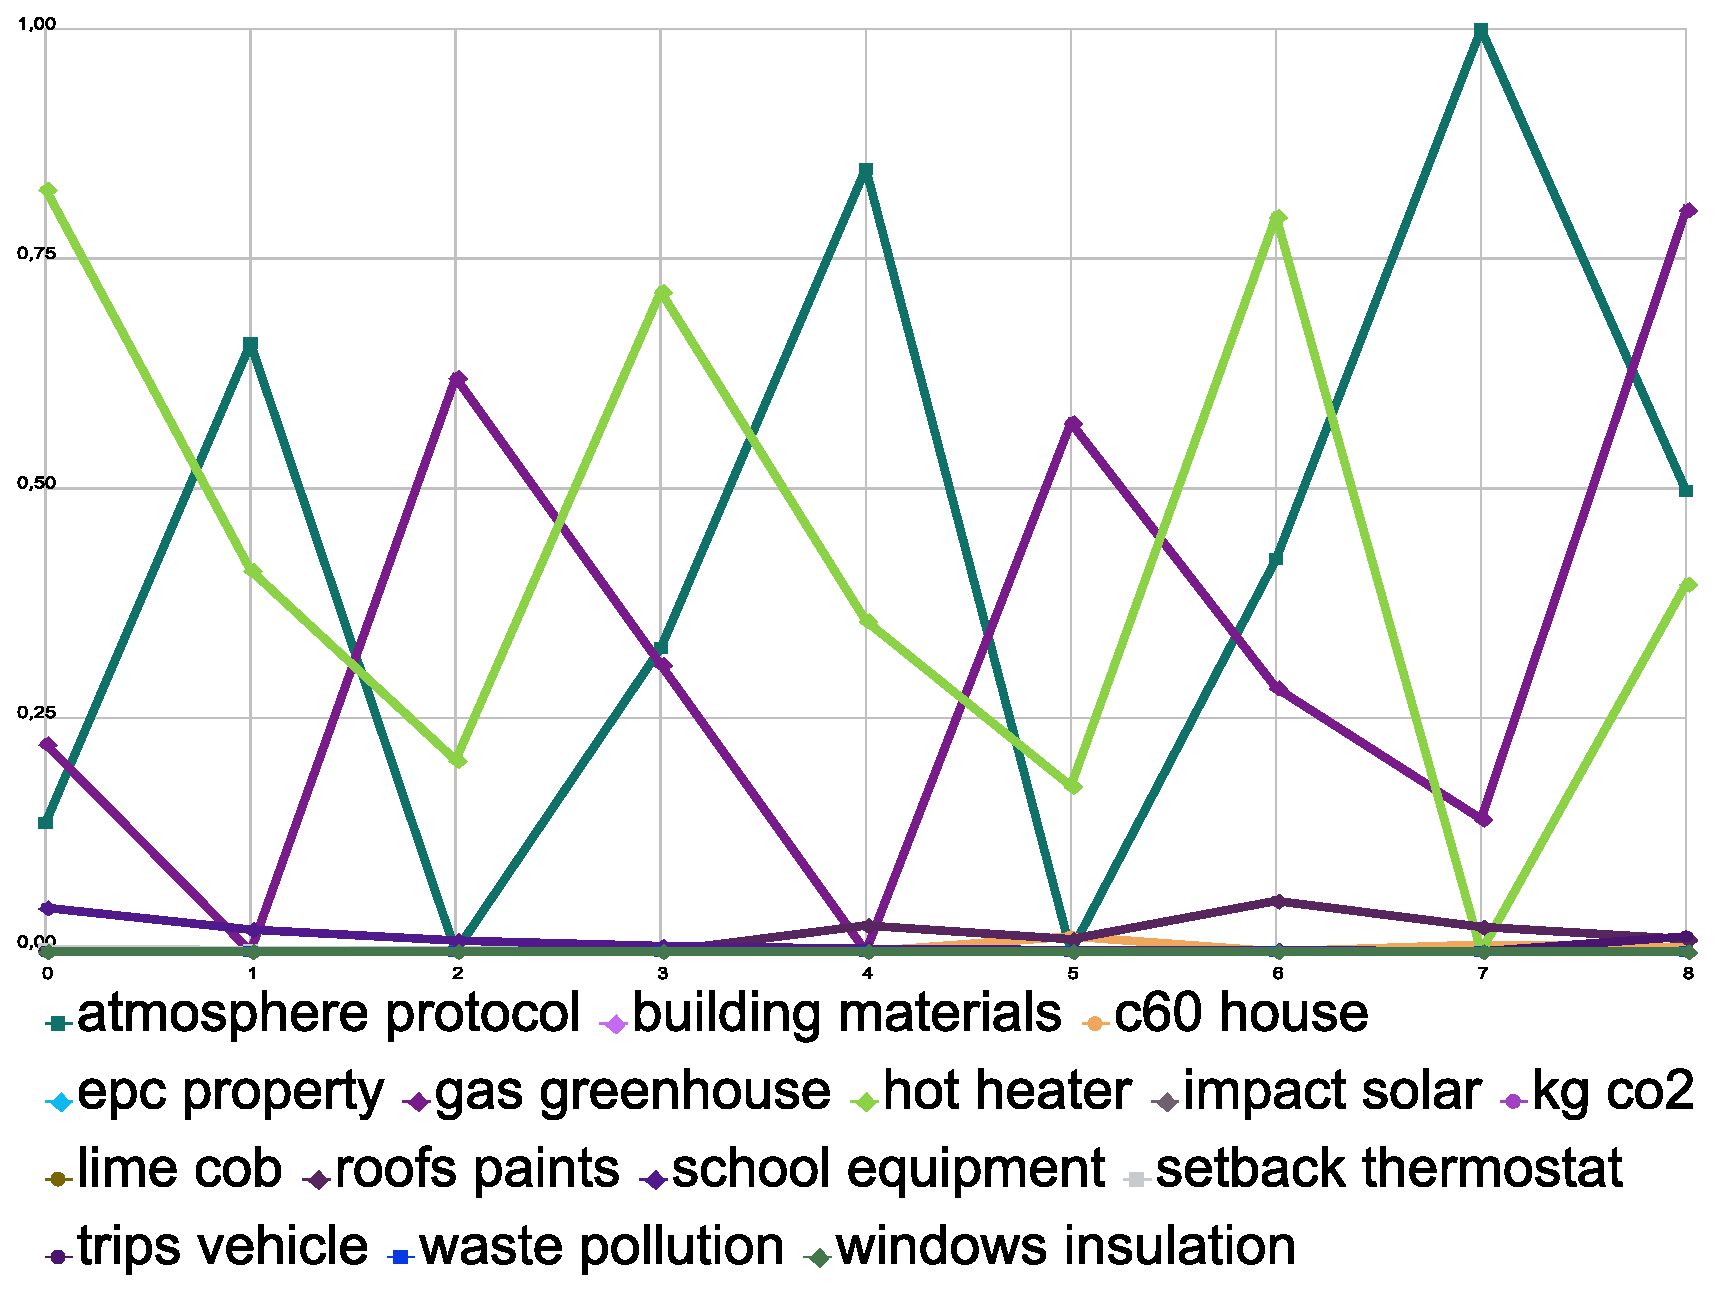
\includegraphics[width=\textwidth]{images/content/06_results/runs/co2_10_3TSw0.2_tpr_betweenness.eps}
\caption{Verlauf für synthetisch erzeugten Dokumentensequenz. Der künstlich erzeugte Verlauf wurde für ein Themenmodell mit 15 Themen erstellt und ist vom Typ \textit{3TSw 0.2}.}
\label{fig:co2_10_3TSw0.2_tpr_betweenness}
\end{figure}

\subsection{Schlussfolgerung}
Aus der Bewertung der Zentralitätsindizes in Abhängigkeit vom verwendeten Algorithmus zur Erstellung der Graphen lässt sich folgendes feststellen.y Das geeignetste Zentralitätsmaß ist die Betweenness-Zentralität. Welcher Algorithmus benutzt werden sollte, um die Graphen aus der Themenkookkurrenz aufzubauen, hängt von der verwendeten Zentralität ab. Aufgrund der Ergebnisse der Bewertung ist es für die Betweenness und die Closeness-Zentralität unerheblich, welcher Algorithmus gewählt wurde. Die visuelle Inspektion der nachfolgenden realen Verläufe zeigt jedoch, dass die letzten beiden Algorithmen visuell bessere Ergebnisse liefern. Für die restlichen Zentralitätsindizes zeigt sich, dass der Algorithmus \CDC$\;$und \TPR$\;$ bessere Ergebnisse liefert als der erste. 

Mit welchen Parametern das Themenmodell trainiert werden soll, lässt sich aus den Bewertungen nicht ermitteln. Für die SCY-Daten weichen die Bewertungen für die verschiedenen Modellsätze so wenig voneinander ab, dass hier gar keine Aussage getroffen werden kann und für die dpa-Text lässt sich nur feststellen, dass eine Stammformreduktion ohne Entfernen der Stopwörter die schlechtesten Ergebnisse geliefert hat. Dies lässt sich jedoch nicht verallgemeinern und hängt zu großen Teilen vom zugrundeliegenden Korpus ab. 

\begin{figure}[ht]
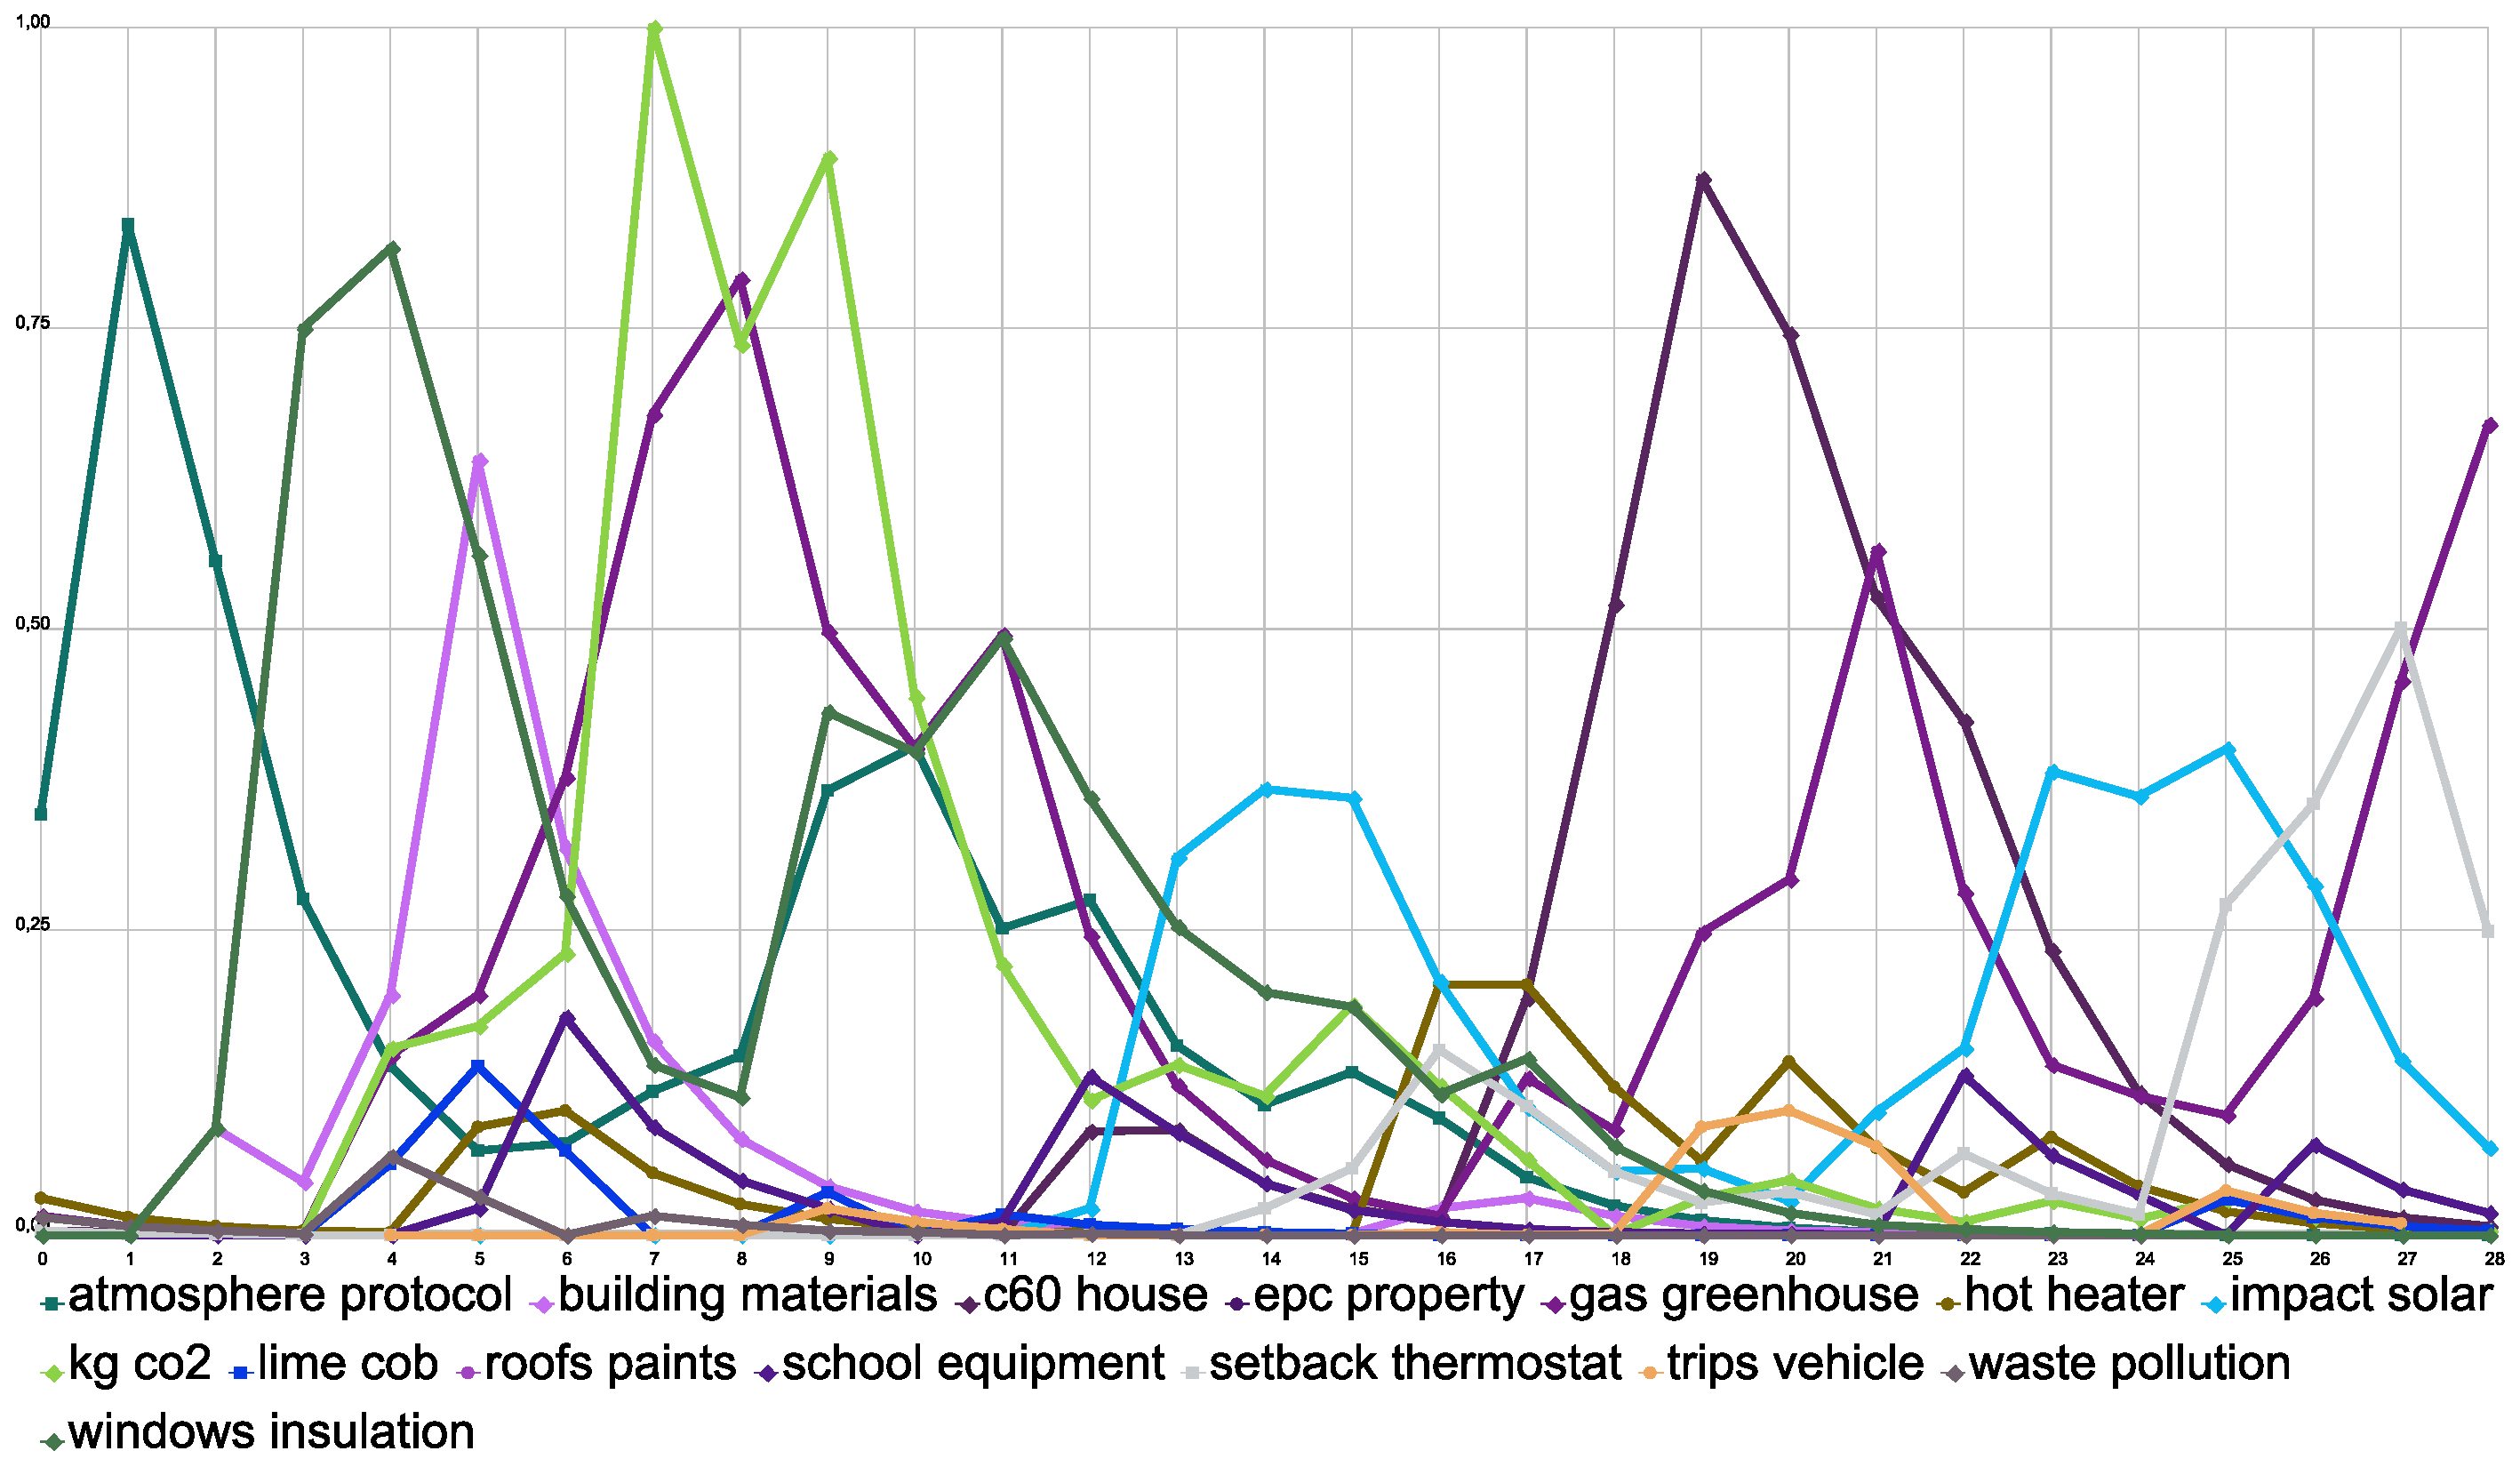
\includegraphics[width=\textwidth, height=0.45\textheight]{images/content/06_results/runs/co2_f7i2_15nostem_tpr_betweenness.eps} 
\caption{Verlauf der Betweenness-Zentralität. Das zugrundeliegende Themenmodell wurde mit 15 Themen mit Entfernung der Stopwörter aber ohne Reduktion der Terme auf ihre Stammform trainiert. Der Verlauf wurde mit dem Algorithmus \TPR$\;$erzeugt.}
\label{fig:co2_f7i2_15stem_tpr_betweeness}
\end{figure}

\section{Anwendungsphase}

Ausgehend von den in Abschnitt \ref{sec:tmValResults} und Abschnitt \ref{sec:centralityResults} vorgestellten Ergebnissen werden nun die realen Verläufe aus dem SCY-Projekt und den dpa-Nachrichtenmeldungen dargestellt. Die Verläufe wurden mit verschiedener Framegröße und Überlappung generiert. Es werden exemplarisch einige Verläufe gezeigt.

\subsection{SCY Chatdaten}
Für die SCY-Chatdaten wurde eine Framegröße von sieben und eine Überlappung von zwei benutzt. Diese Werte wurden experimentell ermittelt und ergaben die besten Ergebnisse. In allen Abbildungen ist auf der X-Achse die Framenummer abgetragen und auf der Y-Achse die normalisierten Zentralitätswerte. Es wird nur ein Verlauf für beide Methoden der Visualisierung dargestellt. Dies zeigt die Unterschiede und Vor- und Nachteile der beiden Arten der Visualisierung.

In Abbildung \ref{fig:co2_f7i2_15stem_tpr_betweeness} sind die Verläufe der Themen für die SCY-Chatdaten dargestellt. Durch die Natur der Chattexte wechseln sich viele Themen sehr schnell ab. Man kann aber erkennen, dass in den Frames 0 bis 10 über die Isolation von Häusern, die dazu verwendeten Baumaterialien und die Auswirkungen auf die \COTWO-Neutralität gesprochen wird. In den Frames 10 bis 17 sind die Themen über Sonneneinstrahlung und Isolation vorherrschend. Ab Frame 18 wird sich hauptsächlich über die Reduzierung von Emissionen und den Zusammenhang zwischen Treibhauseffekt und Sonneneinstrahlung und die Auswirkungen auf die Temperatur gesprochen. Die restlichen Themen treten hier in den Hintergrund.

In Abbildung \ref{fig:co2_f7i2_15stem_tpr_betweeness_seperated} sind die Themen einzeln dargestellt. Für diese Verläufe bietet sich die einzelne Darstellung an, da so differenzierter festgestellt werden kann, über welche Themen gesprochen wird und nicht ganz so wichtigen Themen, nicht in den Hintergrund gedrängt werden.

\begin{figure}[ht]
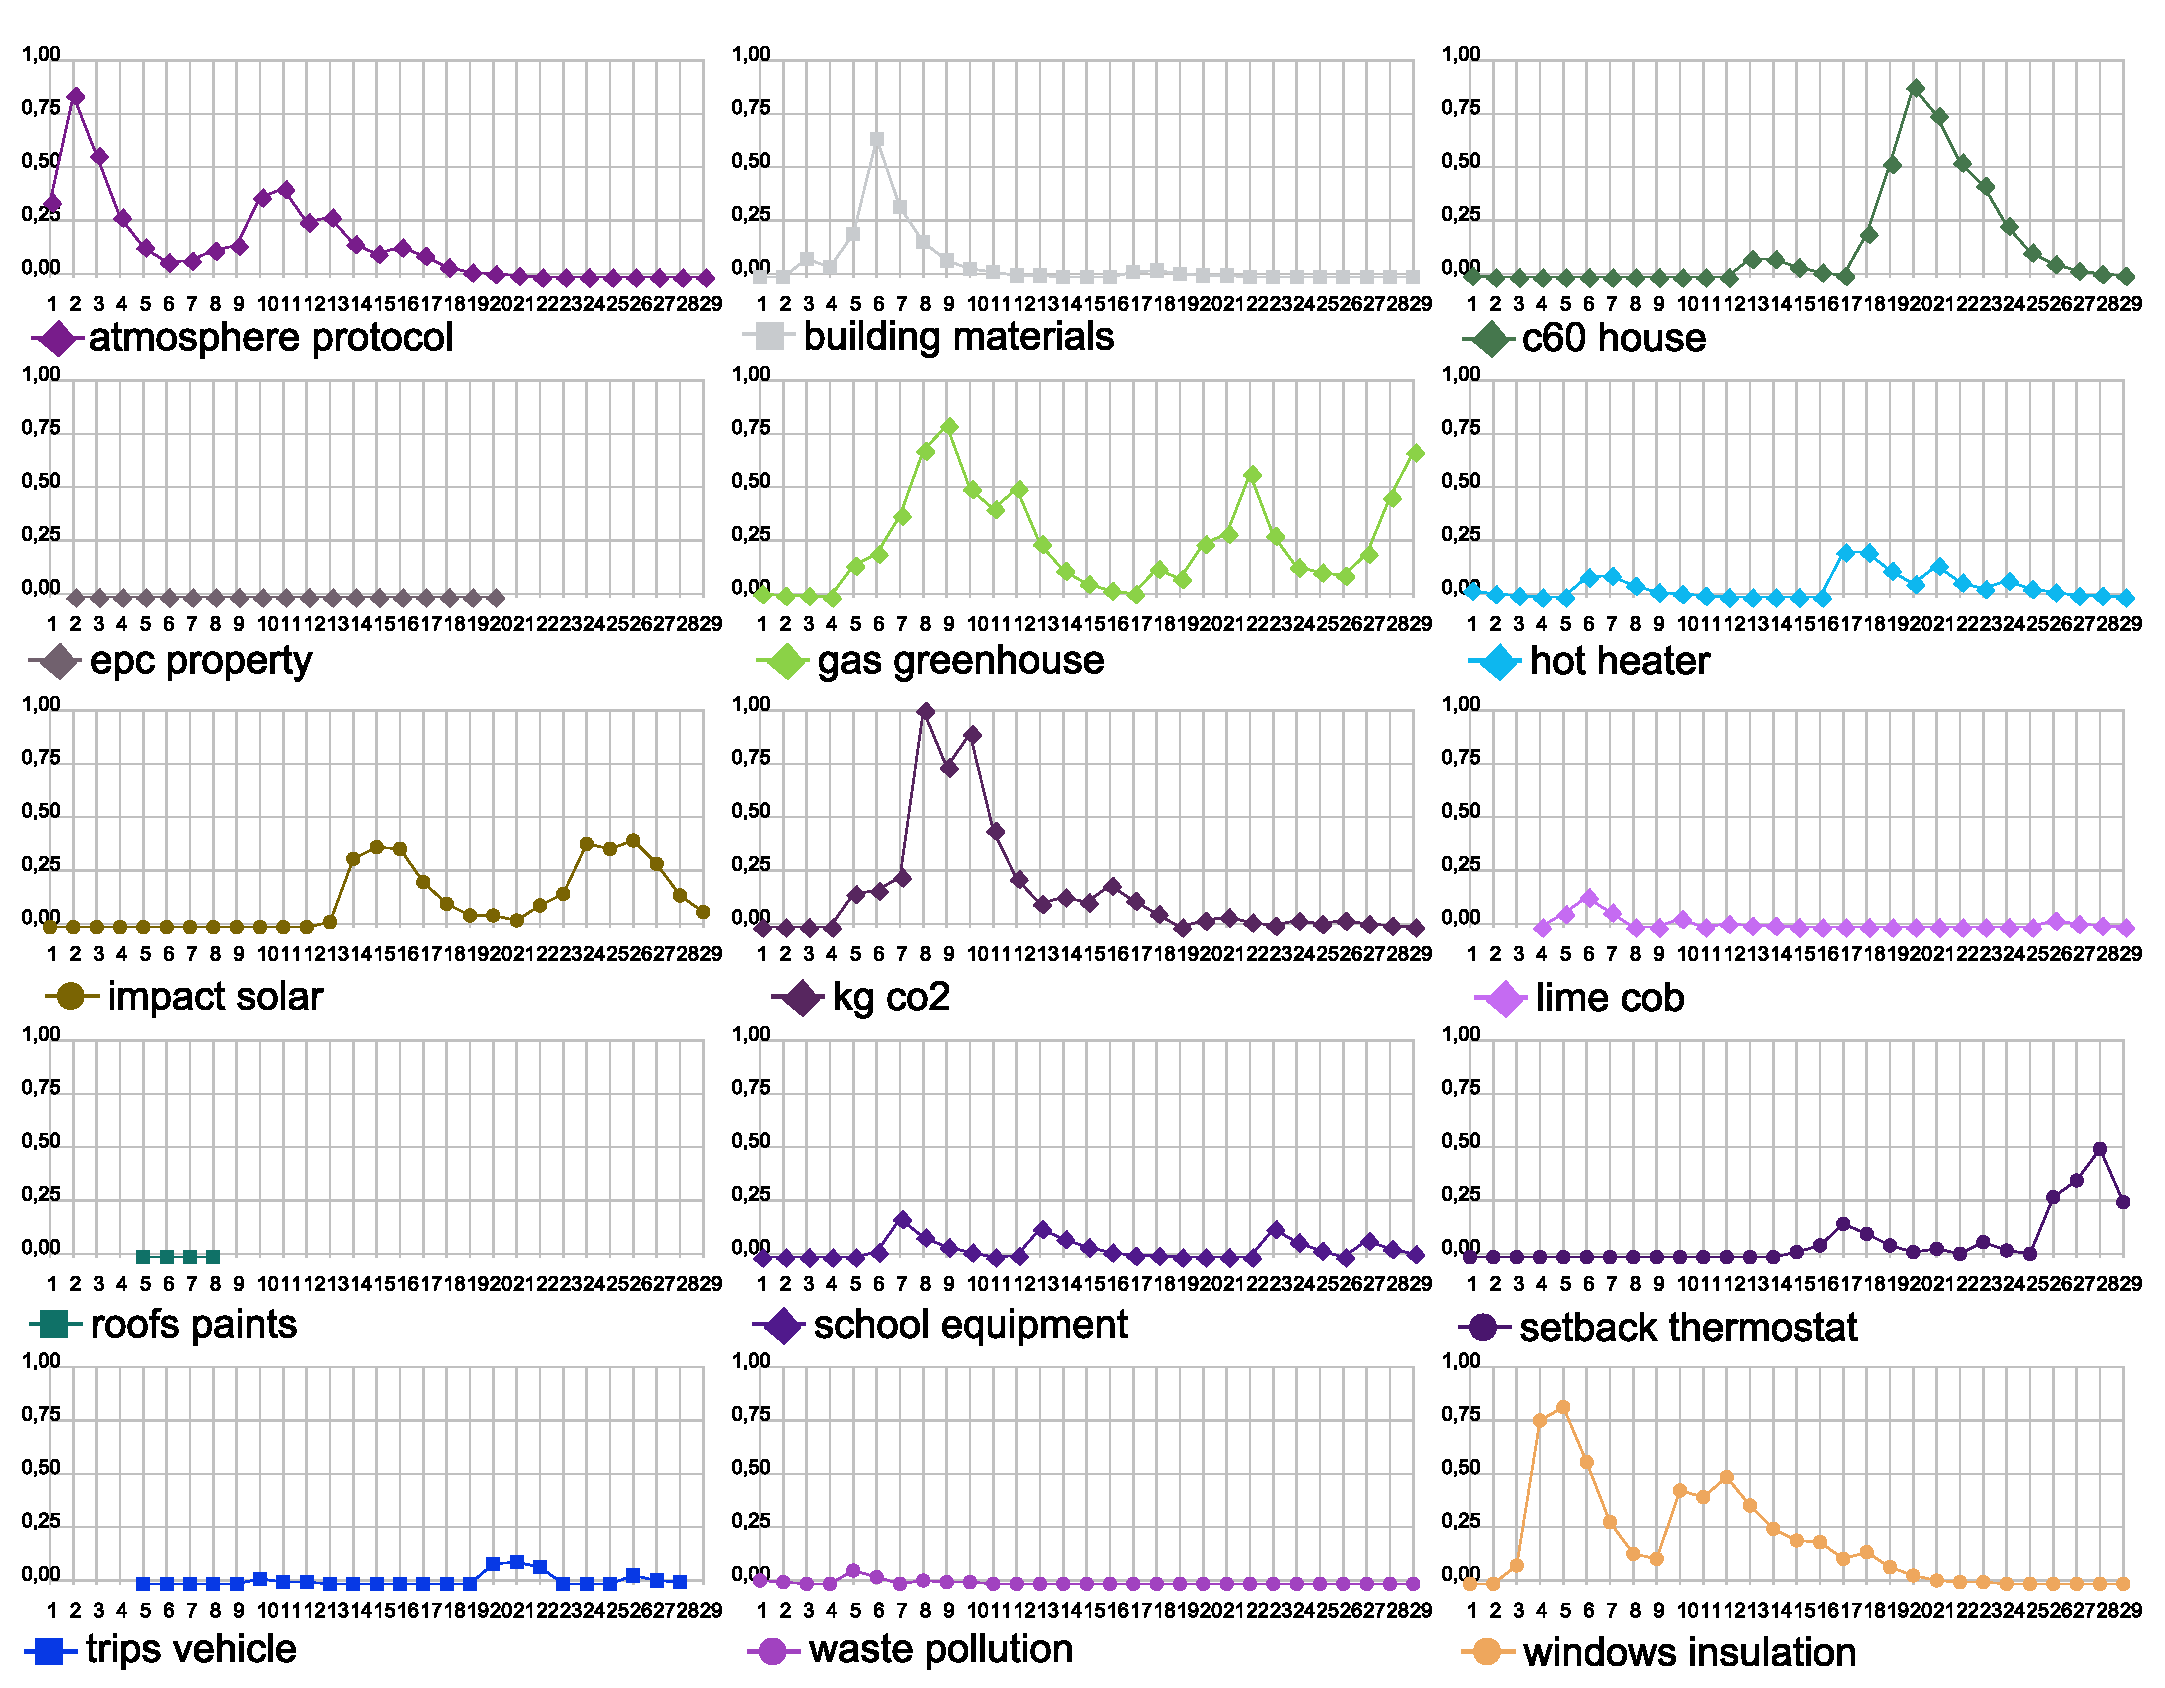
\includegraphics[width=\textwidth]{images/content/06_results/runs/co2_f7i2_15nostem_tpr_betweenness_seperate.eps} 
\caption{Die zu Abbildung \ref{fig:co2_f7i2_15stem_tpr_betweeness} entsprechende separate Darstellung der Themenverläufe. Hier können die moderat wichtigen Themen besser erkannt werden.}
\label{fig:co2_f7i2_15stem_tpr_betweeness_seperated}
\end{figure}

\subsection{dpa Nachrichtenmeldungen}
Für die dpa-Nachrichtenmeldungen wurde zum einen eine Framegröße von 100 mit einer Überlap"-pung von 50 gewählt und zum anderen eine Framegröße von 50 und eine Überlap"-pung von 25. Die Verläufe für verschiedenen zugrundeliegenden Modelle unterscheiden sich nicht sehr stark und es wird deshalb auf die Präsentation der Verläufe für unterschiedliche Modelle verzichtet.
\begin{figure}[ht]
\centering
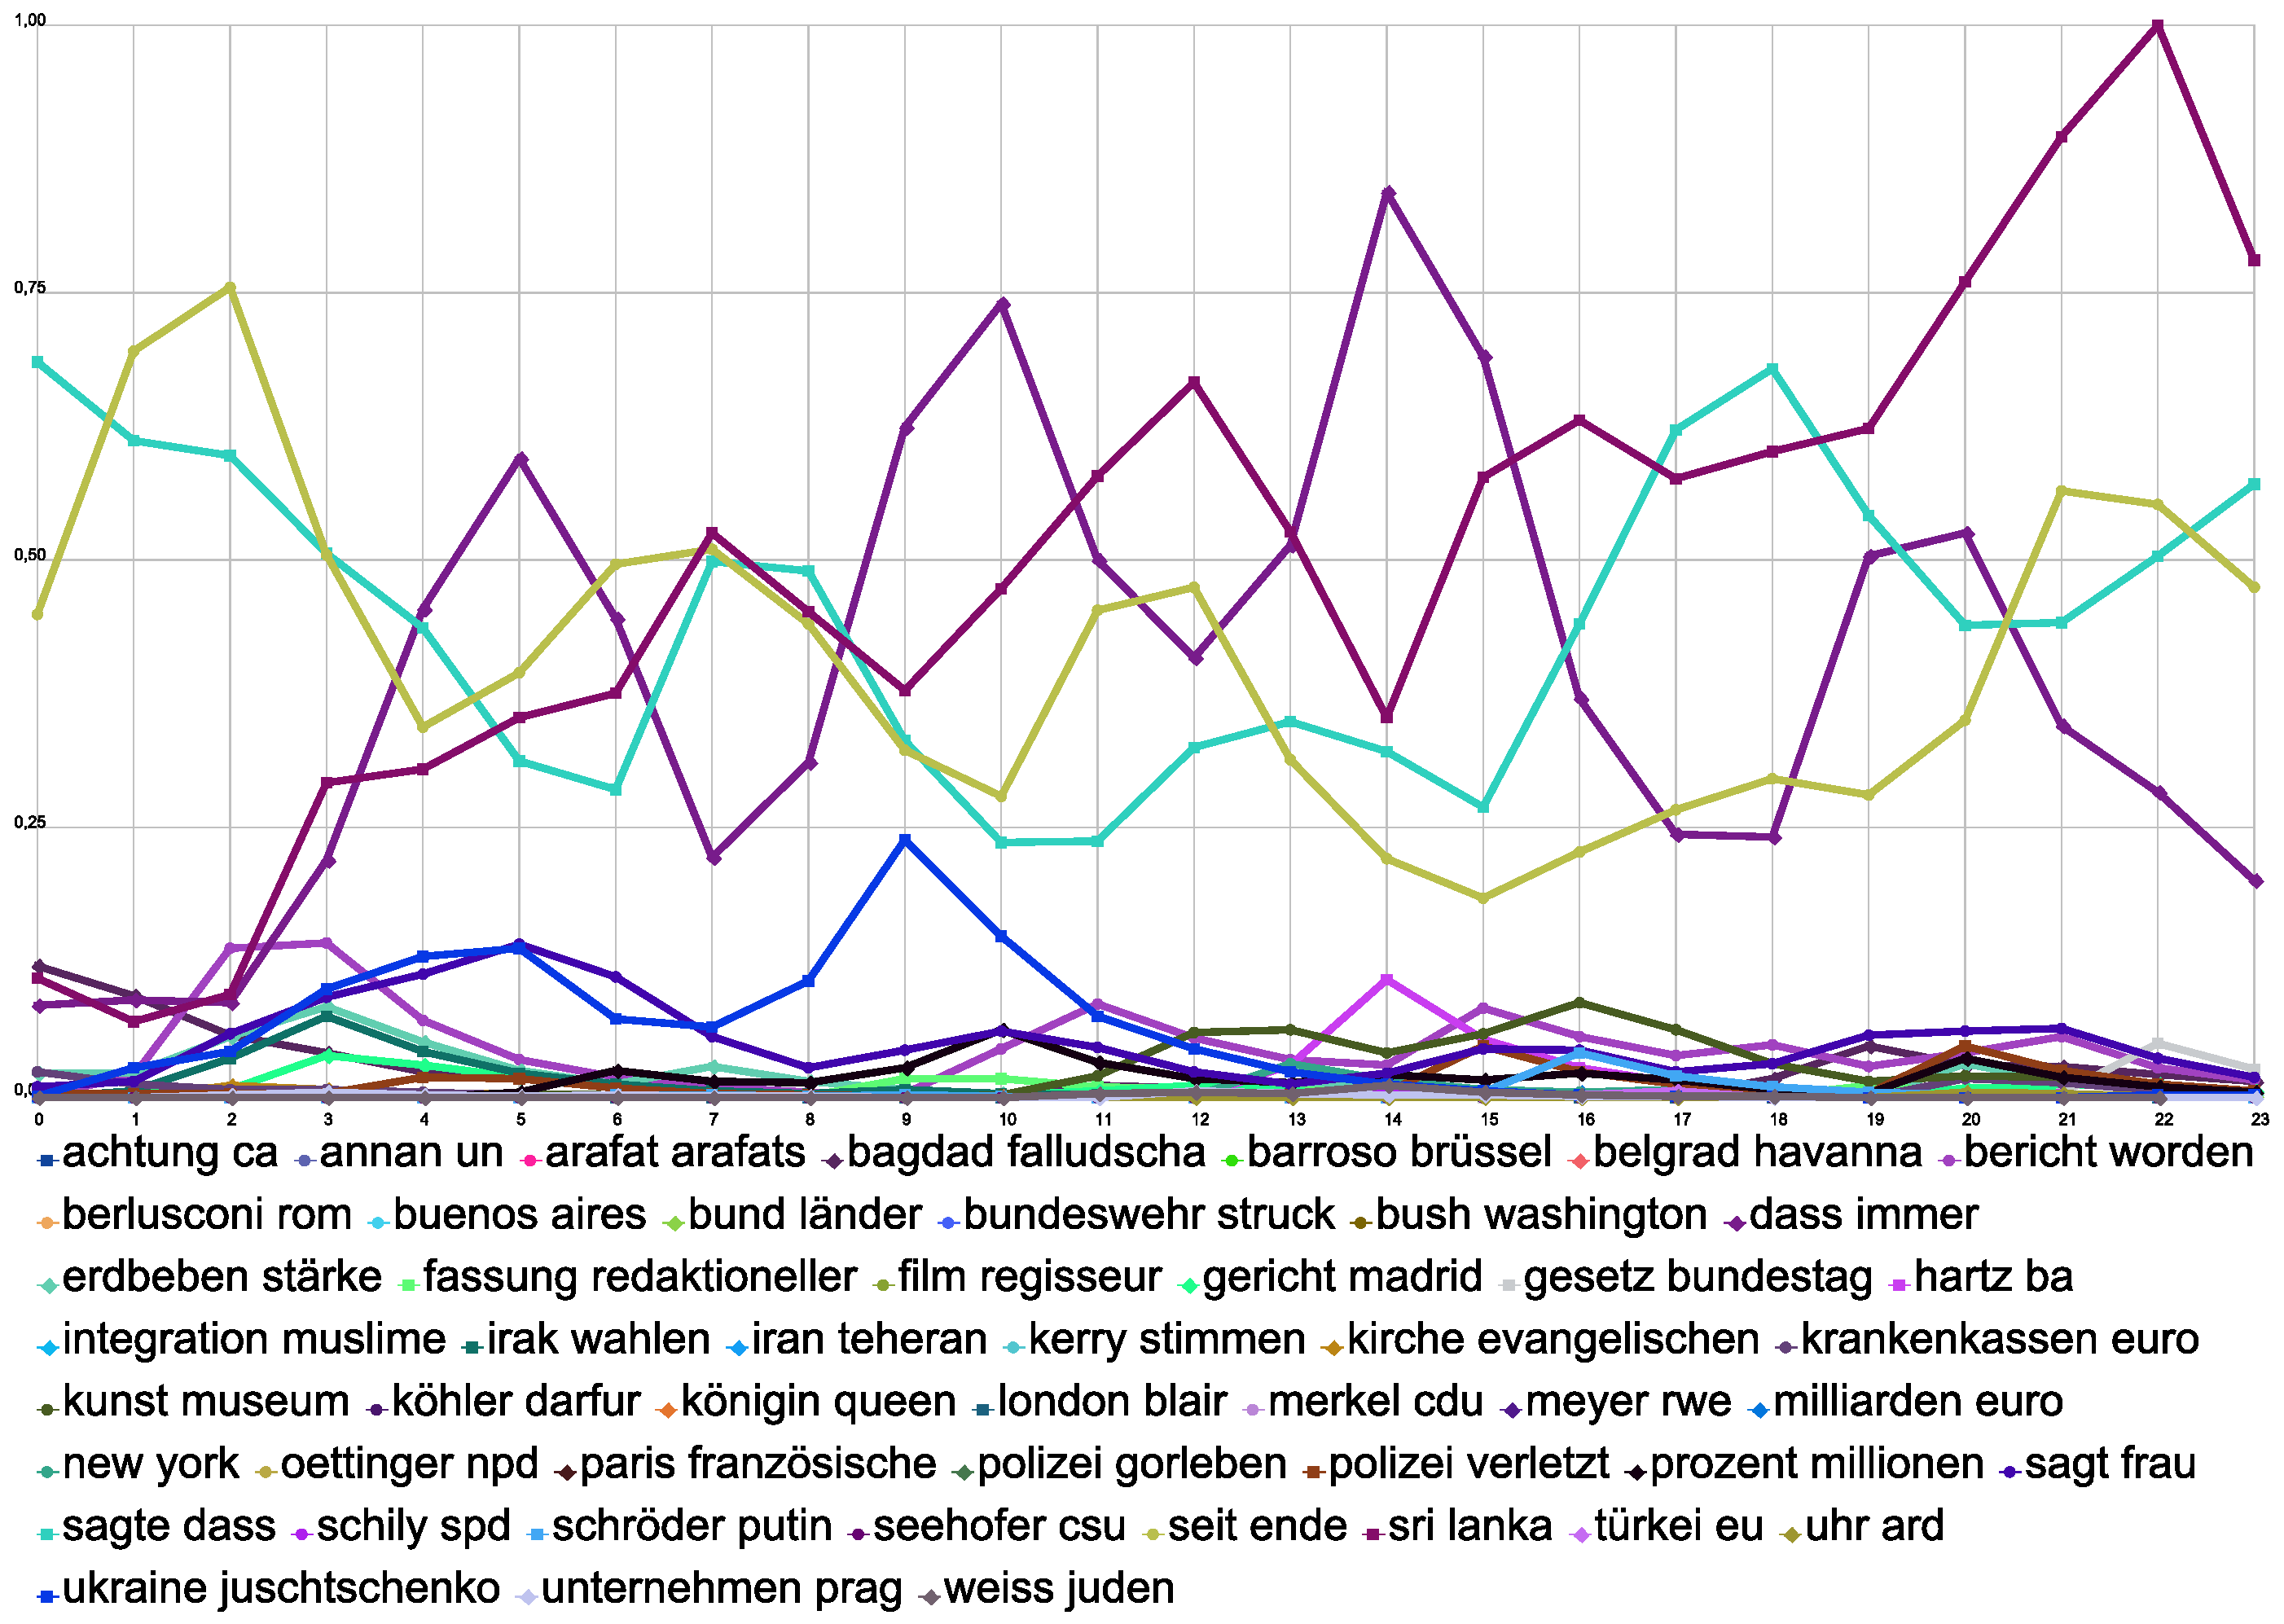
\includegraphics[width=\textwidth]{images/content/06_results/runs/dpa_f100i50_50nostem_betweenness.eps} 
\caption{Themenverläufe der Betweenness-Zentralität für ein Themenmodell mit 50 Themen, ohne Stammformreduktion, mit Entfernung der Stopwörter. Die Framegröße wurde auf 100 gesetzt und die Überlappung auf 50. Die Verläufe wurden mit dem Algorithmus \TPR$\;$erstellt.}
\label{fig:dpa_f100i50_50nostem_tpr_betweenness}
\end{figure}

Wie erwartet, wird das Thema über das Erdbeben in Südasien in beiden Verläufen erkannt und ist sehr präsent. Am Anfang ist es wenig bis gar nicht präsent und steigt dann stark an und bleibt bis zum Ende des untersuchten Zeitraumes im Fokus. Die restlichen drei präsenten Themen sind Themen, die  Terme gruppieren, die inhaltlich keinem anderen Thema zugeordnet werden konnten. Sie bestehen meist aus Funktionswörtern, die in allen Dokumenten auftreten. Da diese Funktionswörter auch häufig in den Texten auftreten, aus denen die Verläufe erstellt werden, wird den Themen, zu denen die Funktionswörter gehören, eine hohe Zentralität zugewiesen und sie erscheinen somit als wichtig. In Abbildung \ref{fig:dpa_f50i25_50nostem_tpr_betweenness} wurden diese Funktionsthemen ausgeblendet, damit man den Verlauf des Themas über das Erdbeben besser erkennen kann. Dieser Verlauf unterscheidet sich vom Verlauf in Abbildung \ref{fig:dpa_f100i50_50nostem_tpr_betweenness}, da eine andere Framegröße benutzt wurde.

\section{Zusammenfassung}
Es wurden die Ergebnisse der entwickelten Methode und deren Anwendung auf verschiedene Korpora dargestellt. Im ersten Teil wurden Themenmodelle bewertet und die am besten bewerteten wurden für die spätere Analyse ausgewählt. Anhand der ausgewählten Modelle, wurden synthetische Dokumentströme erzeugt anhand derer Themenverläufe bestimmt wurden. Diese künstlichen Verläufe konnten darauf untersucht werden, wie gut sie mit den verschiedenen Zentralitätsindizes in Kombination mit den Graphenalgorithmen erfasst werden. Dies ist möglich, da die Dokumentensequenz aus dem Themenmodell generiert wurden und somit das Thema und dessen Wahrscheinlichkeit innerhalb eines Dokuments bekannt sind. Anhand der Textströme konnte man vorhersagen, wie die Verläufe aussehen und somit konnte auch bewertet werden, wie gut sie durch die Zentralitäten erfasst werden. 

Die Betweenness-Zentralität zusammen mit den Algorithmen \CDC$\;$und \TPR$\;$hat sich dabei als am besten geeignet erwiesen. Mit dieser Zentralität und dem Graphenalgorithmus \TPR$\;$ wur"-den für reale Dokumentströme aus dpa-Nachrichten"-meldungen und SCY-Chats Themenverläufe erstellt. Die dpa-Nachrichten"-meldungen enthielten ein bekanntes Ereignis, welches auch korrekt erkannt wurde. Für die SCY-Chatdaten war im Voraus kein einzelnes Ereignis bekannt, jedoch konnten die Diskussionsthemen verfolgt werden. 

\begin{figure}[!ht]
\centering
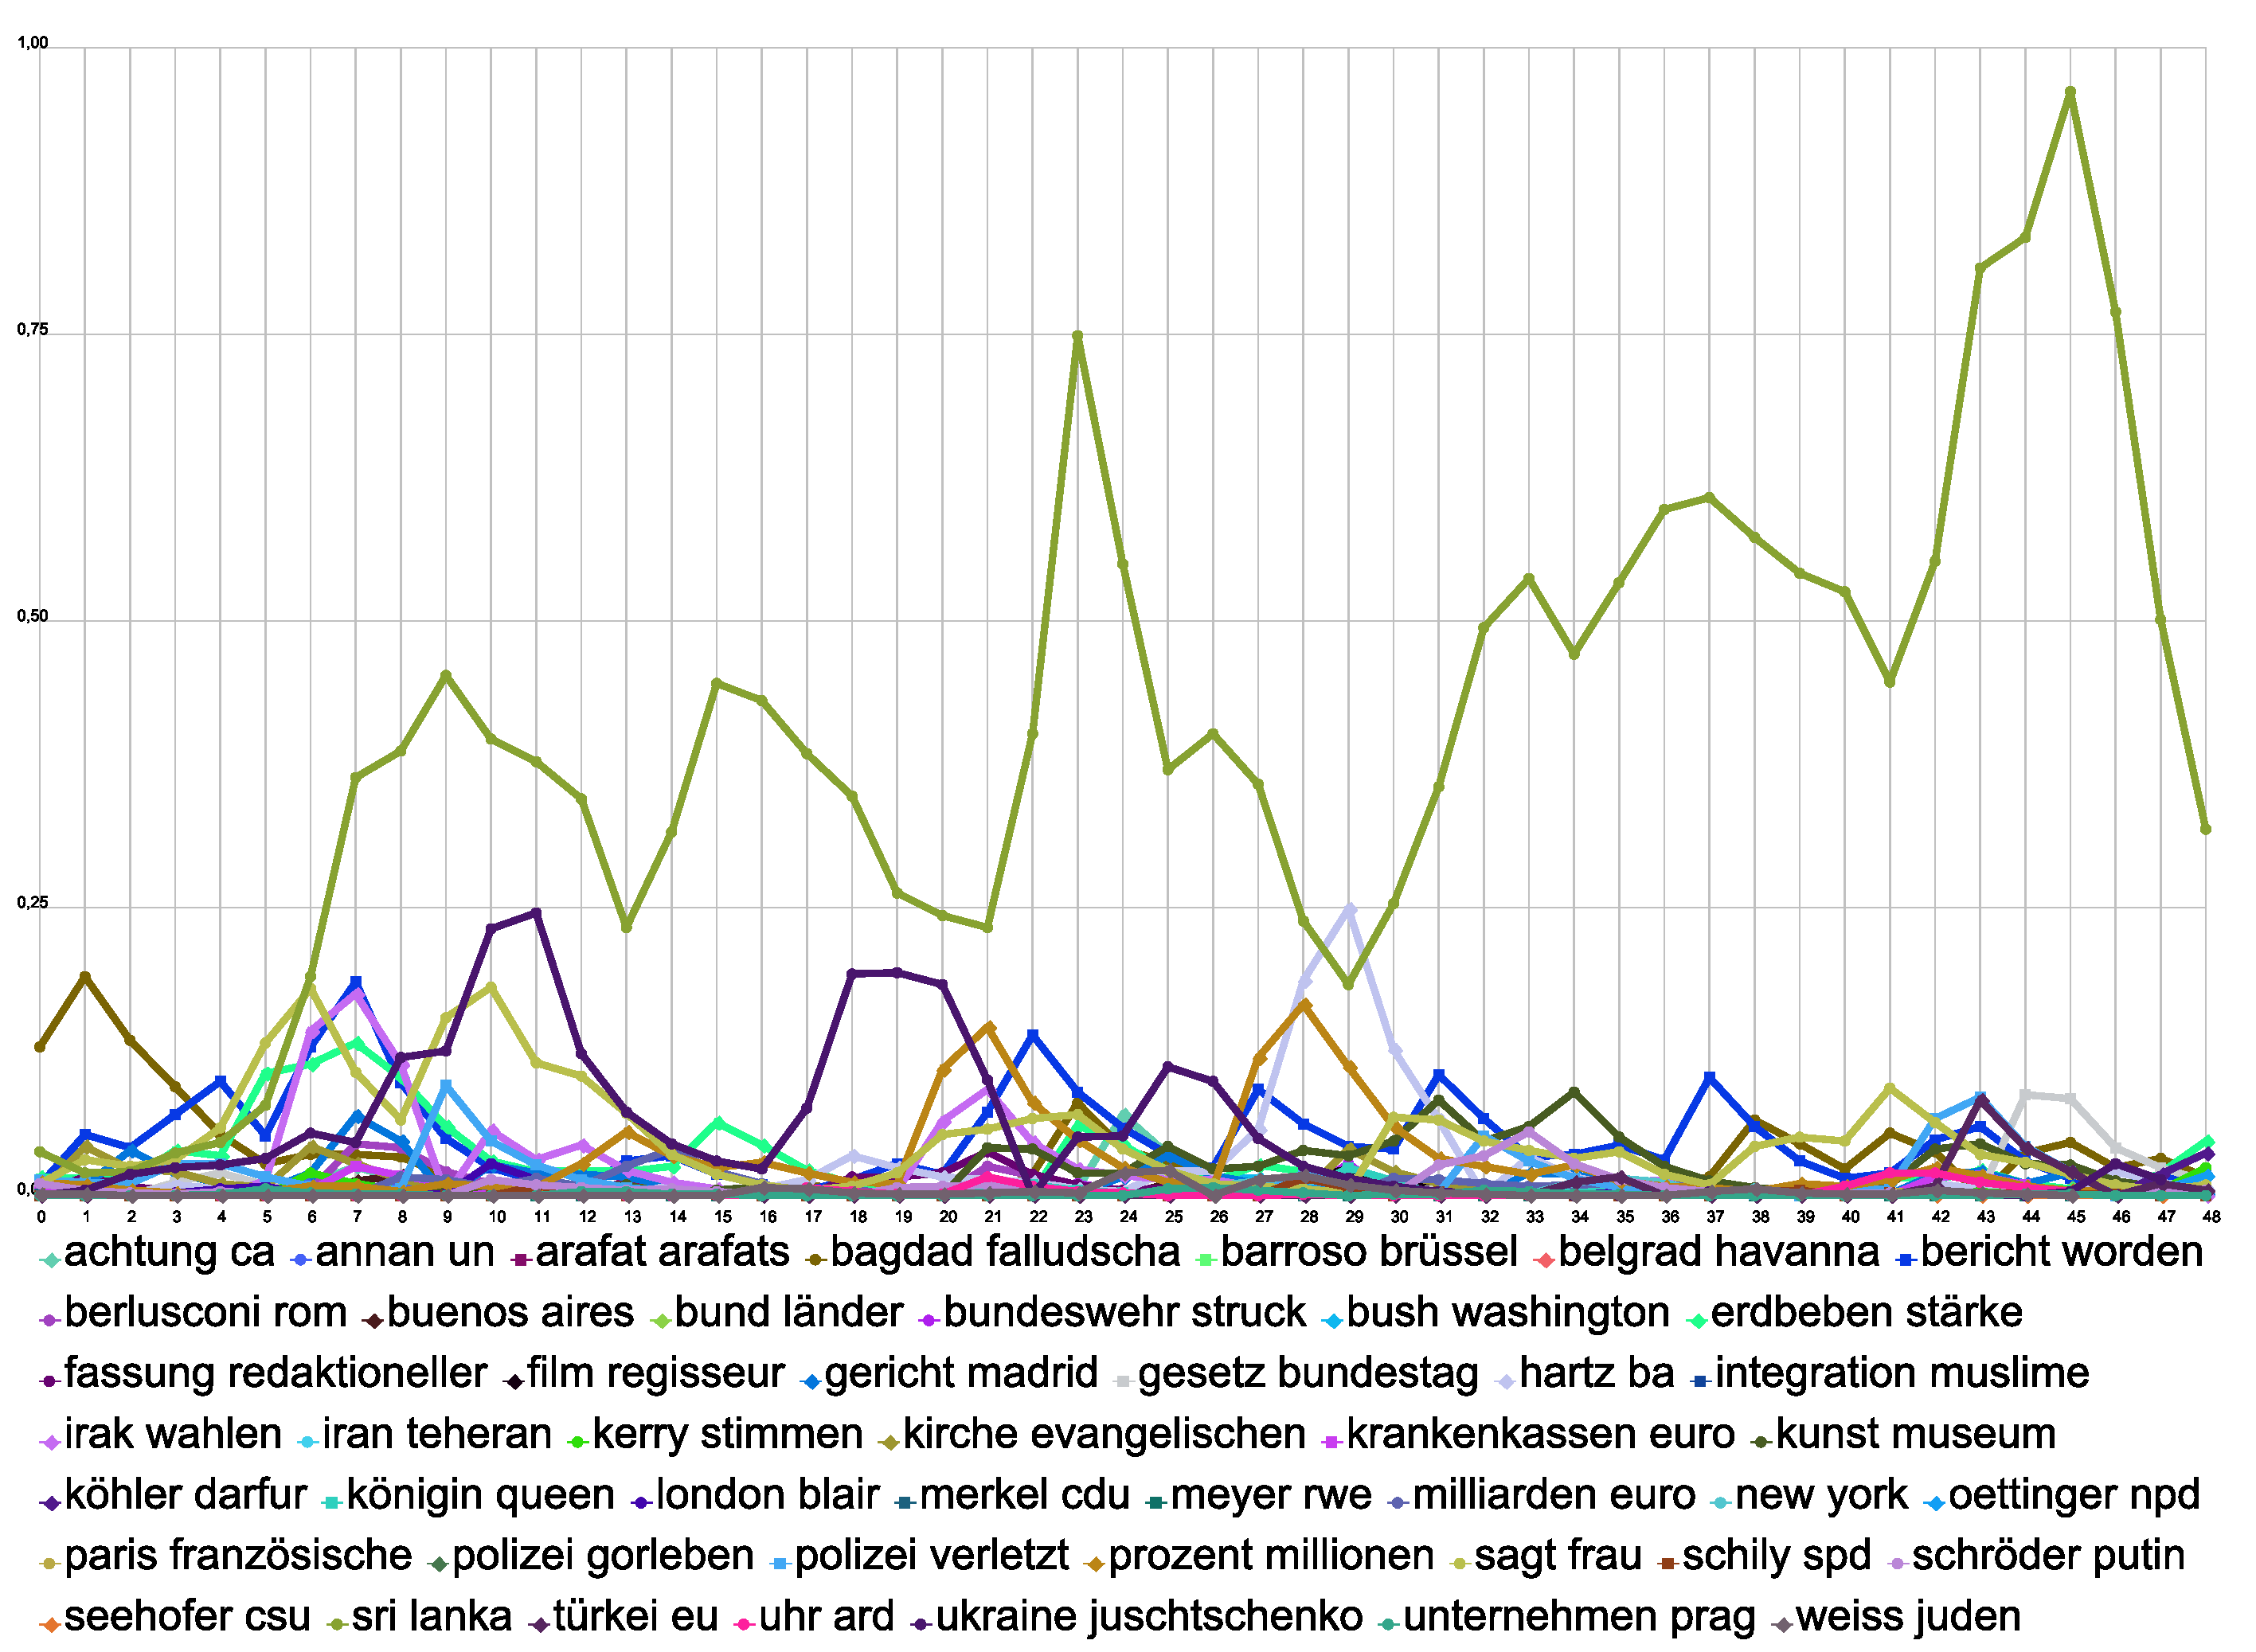
\includegraphics[width=\textwidth, height=0.45\textheight]{images/content/06_results/runs/dpa_f50i25_50nostem_betweenness.eps} 
\caption{Themenverläufe der Betweenness-Zentralität für ein Themenmodell mit 50 Themen, ohne Stammformreduktion, mit Entfernung der Stopwörter. Die Framegröße ist 50 und die Überlappung 25. Die Verläufe wurden mit dem Algorithmus \TPR$\;$erstellt.}
\label{fig:dpa_f50i25_50nostem_tpr_betweenness}
\end{figure}
